% JAC v7 (2026-09-14) — compendium release v2.1 (Zenodo 10.5281/zenodo.22747669; concept 10.5281/zenodo.22051030; supersedes v2.0). US-centric refocus + UKHSA external comparator. Source repository: https://github.com/Nyx-Dynamics/doxypep-bystander
% JAC Original Article — portable/journal-agnostic LaTeX source.
% TEMPLATE_PENDING: no official JAC/OUP LaTeX class was supplied; migrate this
% source into the official template when obtained. House style verified against
% JAC_IFA.rtf (Instructions to Authors): British spelling; methicillin (not
% meticillin); MIC in mg/L; sequential superscript references; structured
% synopsis (Background optional / Objectives / Methods / Results / Conclusions),
% 250 words; main text (Introduction–Discussion) <= 3500 words; Funding and
% Transparency declarations sections required; figures 88 mm / 180 mm with alt
% text under each legend.
\documentclass[12pt,a4paper]{article}
\usepackage[utf8]{inputenc}
\usepackage[T1]{fontenc}
\usepackage{times}
\usepackage{amsmath,amssymb}
\usepackage{graphicx}
\usepackage{booktabs}
\usepackage{tabularx}
\usepackage{rotating} % for sidewaystable
\usepackage[margin=1in]{geometry}
\usepackage{setspace}
\usepackage[right]{lineno}
\usepackage{xurl}
\usepackage[super,sort&compress,comma]{natbib}
\bibliographystyle{vancouver}
\graphicspath{{figures/}}

\doublespacing
\pagestyle{empty} % JAC: do not insert page numbers
\setlength{\parindent}{0.5cm}

\newcommand{\sa}{\emph{S.~aureus}}
\newcommand{\Sa}{\emph{Staphylococcus aureus}}

\begin{document}

% ---------- TITLE PAGE ----------
\begin{center}
{\Large\bfseries Guidance and surveillance capability for bystander \Sa{}
tetracycline resistance under doxy-PEP: a three-stream evidence audit}\\[1.2em]
\end{center}

\noindent A. C. \textsc{Demidont}*\\[0.6em]
\noindent Nyx Dynamics, LLC, Fairfield, Connecticut, USA\\[0.6em]

\noindent\textbf{Running title:} Surveillance and doxy-PEP bystander \sa{} resistance\\[0.6em]

\noindent*Corresponding author. Nyx Dynamics, LLC, Fairfield, Connecticut, USA.
Tel: +1-215-901-2366. E-mail: acdemidont@nyxdynamics.org\\
\noindent ORCID: 0000-0002-9216-8569

\vspace{1.5em}

% ---------- SYNOPSIS ----------
\noindent\textbf{\large Synopsis}

\smallskip
\noindent\textbf{Background.} Doxycycline post-exposure prophylaxis (doxy-PEP)
prevents bacterial sexually transmitted infections and has scaled into guidance
internationally. Doxycycline also selects tetracycline resistance beyond its
target, and \Sa{}---a commensal and pathogen for which doxycycline is one of a
limited number of oral options---is the natural bystander.

\noindent\textbf{Objectives.} To determine whether the guidance and surveillance
deployed around doxy-PEP could follow the bystander-resistance signal the pivotal
trial's final analysis resolved, rather than to estimate a population effect.

\noindent\textbf{Methods.} A reproducible, public-data audit of three evidence
streams---clinical trials, governmental guidance and deployed US
surveillance---each scored against one detectability framework: the within-exposed relative
risk it could detect, benchmarked to an empirical colonisation estimate.

\noindent\textbf{Results.} The final randomised DoxyPEP analysis reported a
3.89-fold higher hazard of incident doxycycline-resistant \sa{} under doxy-PEP
(95\% CI 1.42--10.68; 68 of 393 versus 5 of 163 incident events), with no effect
on colonisation clearance. Yet 0 of 6 outbreak-matched governmental guidelines (0 of 10 coded)
required \sa{} monitoring, and 0 of 12 established US surveillance systems linked
doxy-PEP exposure to an \sa{} tetracycline phenotype at a common population
denominator. Under realistic exposure density and isolate volumes, an ordinary
population system would need an implausible within-exposed effect
(RR~$\approx$~6--28) to move a rate.

\noindent\textbf{Conclusions.} The upstream trial generated information the
downstream architecture is not built to receive. Following the signal requires
sentinel surveillance linking doxy-PEP exposure to the \sa{} tetracycline
phenotype at a common denominator. No population-level causal claim is made.

\vspace{1em}
\linenumbers

% ---------- INTRODUCTION ----------
\section*{Introduction}

Doxycycline post-exposure prophylaxis (doxy-PEP) substantially reduces bacterial
sexually transmitted infections (STIs) and has moved quickly from trial result
into guidance at every level, from the World Health Organization through national
and municipal health departments.\cite{luetkemeyer2023,cdc2024doxypep} Every dose
is selective pressure, and not only on the organisms it targets. \Sa{} is the
consequential bystander: it colonises the anatomical sites these trials swabbed
and carries mobile tetracycline resistance determinants.\cite{grossman2016} For
two decades, community MRSA in these networks has been documented not as
steady-state carriage but as clustered, outbreak-pattern transmission, with the
USA300 lineage moving through sexual networks in San Francisco, Tokyo and
Chicago.\cite{diep2008,dejong2025} The organism colonising these networks is the
same one carried on skin community-wide, so resistance selected within the
network could, if transmitted, extend beyond it. Tetracycline-resistant USA300
was in fact documented in an MSM-predominant community health population two
decades ago, although by the doxycycline-sparing \emph{tet}(K) mechanism, with
those isolates remaining doxycycline-susceptible.\cite{han2007} Doxycycline is
one of a limited number of oral options for outpatient skin and soft-tissue
infection, a choice often made empirically before any methicillin result
returns,\cite{stevens2014,liu2011} so tetracycline susceptibility can matter
clinically before methicillin status is known.

Clinicians who prescribe doxy-PEP have registered antimicrobial-resistance
concerns directly, but those concerns have largely been framed around familiar
targets. In a survey of Italian STI-clinic dermatologists, 91.7\% named
methicillin-resistant \sa{} (MRSA) selection as a worry, tied with gonococcal
resistance as the highest-rated concern,\cite{dona2026} while a systematic
review of 1840 healthcare professionals across four countries likewise placed
antimicrobial resistance among the leading concerns about doxy-PEP.\cite{spence2026}
That framing does not capture the full tetracycline-resistance question in
\sa{}. In a military cohort of 168 personnel receiving doxycycline for malaria
prophylaxis, overall tetracycline-class resistance in \sa{} did not increase,
but \textit{tet(M)} determinants were significantly more common among
doxycycline-exposed personnel ($P=0.031$), showing that aggregate susceptibility
can remain stable while the underlying resistance mechanism shifts.\cite{mende2016}

The trial literature has now answered the tetracycline question directly.
In the final DoxyPEP analysis, among participants free of
doxycycline-resistant \sa{} at baseline, doxy-PEP carried a 3.89-fold higher
hazard of incident doxycycline-resistant \sa{} (95\% CI 1.42--10.68; 68/393
versus 5/163; $P=0.0044$), while the hazard of clearing colonisation did not
differ between arms (HR 1.01, 0.69--1.46).\cite{luetkemeyer2025} The trial's
authors called for public-health surveillance of antimicrobial resistance in
\sa{} and other commensals. One national programme has since begun to address that call:
the UK Health Security Agency's 2026 doxy-PEP monitoring plan for England
proposes tetracycline-resistance surveillance in bystander pathogens, naming
\sa{}.\cite{ukhsa2026}

That call defines the present question. We ask not whether doxy-PEP drives
population-level resistance---a claim we do not make---but whether the guidance
and surveillance deployed around doxy-PEP could follow the signal the trial
resolved, at the population level where the clinical stake lies. The clinically
decisive axis is tetracycline (doxycycline) susceptibility used in empirical oral
therapy, not the methicillin axis around which staphylococcal surveillance is
organised. We audit the three places an answer would have to come from---the
trials, the guidance and the deployed surveillance---each against a single
detectability framework.

% ---------- MATERIALS AND METHODS ----------
\section*{Materials and methods}

\subsection*{Ethics}
This study analysed publicly available guidance, surveillance documentation and
aggregate published data; it did not involve individual-level human-participant
data, and institutional review board approval was therefore not required.

\subsection*{Design}
The study is a documentary and quasi-computational audit assembled in three
streams, collected and analysed in sequence: clinical trials (Stream A), the
governmental guidance built on them (Stream B) and the population surveillance
meant to monitor them (Stream C). No individual-level or restricted data were
used; every input is public. Sources were
located, read, coded with page/section/table locators and SHA-256-pinned before
analysis; analysis decisions that could go either way were date-logged before
results were known; and every figure and table regenerates from a single command
over a test-gated pipeline archived with a citable
DOI.\cite{armond2024integrity} Large language model use is disclosed in the Acknowledgements.

\subsection*{Detectability framework}
The three streams were evaluated within a common detectability framework:
whether, and at what effect magnitude, each measurement architecture could
resolve a bystander-resistance signal. For the trial and surveillance streams,
detectability can be expressed quantitatively against an externally specified
relative-risk benchmark; for guidance, the corresponding question is whether
\sa{} measurement is specified at all. The empirical benchmark is Soge
\textit{et al.}\cite{soge2025} (tetracycline-resistant \sa{} colonisation,
18\% versus 8\% in doxy-PEP users with $>$3 doses/month versus non-users;
RR~$\approx$~2.25); a cross-organism gonococcal RR~$\approx$~1.42 is retained
as a prespecified, more conservative secondary benchmark.

Hazard ratio and risk ratio are different estimands, so the trial estimate is
used only as a magnitude reference, not as a numerically equivalent effect
measure.

\subsection*{Sources and coding}
The author identified, retrieved and screened all source documents for
eligibility; each eligible document was then coded from full text against a
prespecified schema, every value carrying a page, section or table locator. For
the guidance corpus (Stream B), a first LLM pass coded all 10 documents against
the schema. A second, blinded pass---run through a chat interface rather than the
command-line agent, but within the same model family---separately re-coded a
5-document subsample (25 field-codings) for reliability. Disagreements were
resolved by the author against the source. Per-field agreement is reported as raw
concordance, which measures the reproducibility of the coding protocol rather than
its accuracy; because the passes share a model family their errors are not
independent, so a Cohen's $\kappa$ is given for context only (Limitations). The surveillance enumeration (Stream C) was
coded by a single pass; its inclusion and exclusion list, with a stated reason
per system, is given in the Supplementary data and reflects systems as deployed
as of August 2026. All coding prompts and outputs are in the public repository.

\subsection*{Stream A---trials}
For each primary-trial \sa{} arm comparison (first-party published data only), we
computed, from arm sizes and observed control rate, the exact (Fisher) power to
detect the externally fixed benchmark effect and the minimum detectable RR at
80\% power; fixing the effect externally makes this a design-based sensitivity
analysis rather than observed power. The \sa{} assay is doxycycline throughout
(E-test, MIC~$\geq$~16~mg/L). We tabulated how the resistance result was reported
across trial venues and secondary syntheses (numerator, denominator basis,
conditioning set and terminology). The final trial performed a participant-level time-to-event analysis itself; we cite that randomised result
directly and did not re-estimate it. Cross-sectional carriage alone does not resolve the
clustered transmission structure of \sa{} in these networks; the supporting
dispersion, trend-test degradation and outbreak-shape analyses are MRSA-scoped
(MRSA being a subset, not the analytic unit) and are reported in the
Supplementary data (available as Supplementary data at \textit{JAC} Online).

\subsection*{Stream B---guidance}
The denominator was anchored to the same clustering
evidence used in Stream A: US jurisdictions with documented community-associated
MRSA/USA300 transmission in men who have sex with men.\cite{dejong2025,diep2008}
We took governmental public-health guidance only (clinic and
provider-organisation documents excluded, with reasons). Each document was coded
from full text, one record per document, every finding carrying a locator, for
whether it requires, suggests or omits \sa{} monitoring and whether it names,
counsels on or measures the organism (coding provenance above). An independence
check separated genuinely independent declines from documents that defer to, or
are adapted from, one another.

\subsection*{Stream C---surveillance}
We examined a prespecified set of 12 established US surveillance and data systems
(federal, state or metropolitan) plausibly capable of capturing, at the required
level, either doxy-PEP/doxycycline exposure or \sa{} AMR phenotype, and coded each
on three capabilities: exposure-side capture,
phenotype-side capture (of the \sa{} tetracycline unit, not the MRSA subset) and
the join, recording the geographic resolution of each side. A supporting analysis
asked whether, even at a common denominator, the exposed subgroup is dense enough
to move a population rate. The exposed population is indexed on the combined PrEP
and people-living-with-HIV male count, the primary specification, because the trial
enrolled both (AIDSVu 2024 state PrEP and prevalence). The dilution fraction is
$f=((\text{male-PrEP}+\text{male-PLWH})\ \text{density}/10^{5})\,\text{uptake}\,d\,\kappa$,
where $d$ is the share of users taking $>$3 doses/month (the subgroup carrying the
benchmark effect) and $\kappa$ the isolate-enrichment factor. Because $f$ tracks
exposure density rather than headcount it is population-independent, and the minimum
detectable change in a proportion near baseline $R_0$ inverts to
$\mathrm{RR_{needed}}=1+\mathrm{MDE}/(f R_0)$. Parameter choices were deliberately mixed: isolate volume was set high to favour detection, while the
realistic under-sampling ($\kappa=0.5$) and dose-threshold ($d=0.5$) factors bound
against it. Both ranges and the resulting $\mathrm{RR_{needed}}$ are reported;
full grids and the metropolitan break-even are in the Supplementary data.

\subsection*{Scope}
The corpus and the surveillance enumeration were restricted by design: Stream~C is
a prespecified set of US systems, and Stream~B is US governmental guidance with the
World Health Organization included only as the international apex reference. The
resulting counts describe US architecture, not a global census.

% ---------- RESULTS ----------
\section*{Results}

\subsection*{Stream A: trial measurement and reporting of the \sa{} endpoint}
The final DoxyPEP
analysis ran the participant-level test the interim had not---time to first
detection of doxycycline-resistant \sa{} by arm, standard-of-care censored at
crossover, by Cox proportional hazards---and returned HR 3.89 (95\% CI
1.42--10.68; $P=0.0044$), with colonisation clearance unchanged (HR
1.01).\cite{luetkemeyer2025} The 2023 interim, by contrast, was presented as reassuring
on a cross-sectional resistance fraction and was underpowered for any externally
specified effect (0 of 4 comparisons powered; minimum detectable RR 3.8--5.1
against the benchmark 1.42--2.25). The hazard ratio is not comparable to that
cross-sectional minimum: the estimand, not the sample size alone, became adequate
to the question.

Two features of the interim reporting remained relevant to downstream interpretation.
First, a unit mismatch: the trial's data table is headed ``phenotypic resistance
to the tetracycline antibiotic class'' while its methods define the \sa{} assay
as doxycycline, and the federal guideline then describes the doxycycline result
as ``tetracycline resistance in \sa{}''.\cite{cdc2024doxypep} Because efflux and
ribosomal-protection mechanisms differ in whether doxycycline still works
(below), an endpoint scored as ``the tetracycline class'' does not answer the
treatment-relevant question. Second, the signal was reported over differing,
incompletely documented denominators and then propagated into secondary reporting
under further contrasts (Table~\ref{tab:propagation}): the resistant numerator
changes from 5 to 16 to 28 and the denominator basis shifts from colonised
carriers to all-swabbed. The percentage therefore propagated more consistently
than the denominator, contrast and terminology needed to interpret it. The individual-level
data that could reconcile these first-party reports are not publicly
available.\cite{luetkemeyer2023}

Across trials the phenotype was measured on incompatible terms: DoxyPEP measured
doxycycline resistance by E-test over two denominators; DuDHS measured it by disc
diffusion in single-digit carriers; DOXYVAC measured only MRSA carriage---a
methicillin, not a tetracycline, quantity, and one that itself rose within the
doxy-PEP arm (1.8\% to 9.9\%) while being reported as a between-arms
null.\cite{vanbaelen2024c} A pooled estimate is not defensible. Even the intensively surveilled gonococcus was phenotyped in fewer than one diagnosis in five (resistance testing unavailable for 83\%, 212/256).\cite{luetkemeyer2023croi}

\begin{table}[t]
\centering
\caption{Changes in reporting of the DoxyPEP \sa{} resistance signal across publication and guidance venues.
Numerators, denominators, conditioning sets, and contrasts differed across reports. The table is intended to show how the reported percentage was propagated while the underlying denominator and estimand changed; rows should not be interpreted as equivalent effect estimates.}
\label{tab:propagation}
\footnotesize
\setlength{\tabcolsep}{4pt}
\renewcommand{\arraystretch}{1.15}
\begin{tabularx}{\textwidth}{@{}
  >{\raggedright\arraybackslash}p{0.16\textwidth}
  >{\raggedright\arraybackslash}p{0.18\textwidth}
  >{\raggedright\arraybackslash}p{0.26\textwidth}
  X@{}}
\toprule
Venue & Reported result & Frame / conditioning set & What travels downstream\\
\midrule
NEJM appendix\cite{luetkemeyer2023} & 5/31 = 16\% & Month-12 doxy-PEP arm; resistant among carriers & Numerator and carrier denominator explicit\\
CROI abstract\cite{luetkemeyer2023croi} & 16/137 = 12\% & Doxy-PEP arm; all-swabbed denominator & Different numerator/denominator basis\\
CDC guideline\cite{cdc2024doxypep} & 28/222 = 13\%; summarised 5\%$\rightarrow$13\% & Doxy-PEP arm; guideline frame & Percentage retained, provenance less transparent\\
JAMA Insights\cite{mayer2023} & 5\% versus 4\% & Doxy-PEP versus control; ``infected with'' & Between-arm percentage only; counts/timepoint dropped\\
JAMA Synopsis\cite{flores2025} & 5\%$\rightarrow$16\% & Within arm, among \sa{}-isolated & Carrier-conditioned within-arm percentage (baseline to month 12)\\
Lancet ID final\cite{luetkemeyer2025} & HR 3.89 (1.42--10.68); 68 of 393 vs 5 of 163 & Participant-level time-to-event; baseline-negative, as-randomised & Not cited by any coded guidance, including two revised after its March 2025 online publication\\
\bottomrule
\end{tabularx}
\end{table}

The estimand shift did not propagate downstream: no guidance document in the
corpus cites the final time-to-event analysis or any hazard ratio, and the two
documents revised after its online publication in March 2025---WHO (2026) and San
Francisco (May 2026)---retained a cross-sectional or generic frame. Non-citation
is telling here because this corpus demonstrably transmits numbers when it has
them: CDC carried the cross-sectional 5\%$\rightarrow$13\% figures and WHO cites
Soge's colonisation estimate.\cite{soge2025}

\subsection*{Stream B: \sa{} monitoring requirements in governmental guidance}
The governmental guidance shows a consistent within-document asymmetry: the
efficacy question received a graded, systematic evidence review, while the
AMR-harm question---explicitly including resistant-pathogen development---received
an ungraded review in the same document. Of the six documented-outbreak
jurisdictions with governmental doxy-PEP guidance (San Francisco, Chicago, New
York City, Boston/Massachusetts, Los Angeles County and San Diego), 0 require or
suggest \sa{} monitoring. The decline is not an artefact of copying: four
jurisdictions are independently authored, one (Los Angeles County) is adapted
from San Francisco and one (Massachusetts) from an external template. Nor is it
for want of naming the organism---three of the six name \sa{} specifically, two
invoke only a generic ``microbiome'' risk and one is silent; even where named,
none measure it. Across the full coded corpus (10 documents: CDC, WHO and eight
US jurisdictions) the result is identical: none require \sa{} monitoring.
Double-coding of a 5-of-10-document subsample (25 field-codings) gave 92\% raw
agreement (23/25); the one field with meaningful disagreement (bystander treatment;
$\kappa=0.58$) is reported unrounded. Providers are nonetheless required to counsel
patients about resistance in commensal organisms---a harm no system measures.

\subsection*{Stream C: surveillance capability and exposure--phenotype linkage}
Following the signal requires one system to carry, at a common population
denominator, both who is exposed to doxy-PEP and what tetracycline phenotype \sa{}
carries. Across this prespecified set of twelve systems, none does
(Figure~\ref{fig:linkage}). Two systems capture exposure at a population
denominator (AIDSVu and CDC AtlasPlus, as a pre-exposure prophylaxis proxy, not
doxy-PEP itself),\cite{aidsvu} and zero capture \sa{} tetracycline resistance at a
population denominator, so population-level linkage is not possible.

The absence is structural, not incidental. Wherever \sa{} is surveilled at a population
denominator the reported axis is methicillin: the one population-based platform,
Active Bacterial Core surveillance/Emerging Infections Program (ABCs/EIP),
reports invasive MRSA; the National Healthcare Safety Network reports MRSA events;
and the only routine source of \sa{} tetracycline susceptibility, the facility
cumulative antibiogram, is non-standardised and carries no population
denominator, because CLSI M39 mandates the MRSA/MSSA split and makes tetracycline
a selectively suppressible supplemental agent. The National Antimicrobial
Resistance Monitoring System excludes \sa{} altogether, and tetracycline-resistant
\sa{} is not nationally notifiable in the United States. A system could be built---most directly by
adding \sa{} tetracycline susceptibility to ABCs/EIP, which already holds the
denominator---but none is deployed.

Nor could an ordinary population system recover the missing side by collecting
more isolates. Indexing the exposed population on the combined PrEP and
people-living-with-HIV male count---the primary specification, because the trial
enrolled both (Materials and methods)---the realistic-cell within-exposed effect
required to move a population rate runs to RR~$\approx$~6--28 across the
design-effect range (Figure~\ref{fig:detect}); the more restrictive PrEP-only
indexing gives RR~$\approx$~14--64, which overstates infeasibility. Either way it
is far above any plausible effect. Detection appears in a single grid cell that
maxes every generous assumption at once ($\mathrm{RR_{needed}}$ 1.03, or 1.79 under
single-comparison inference; parameters in the Supplementary data). Detectability turns on quantities no deployed system reports---exposure density, isolate
enrichment and dosing frequency. Against the more conservative cross-organism
benchmark (RR 1.42), the best metropolitan cell needs about twice the combined male
exposure density of the densest US geography (Washington, D.C.), and realistic
cells far more. The only configuration that restores sensitivity is to sample \sa{}
directly from doxy-PEP-exposed persons, converting surveillance into a sentinel
cohort.

\begin{figure}[t]
\centering
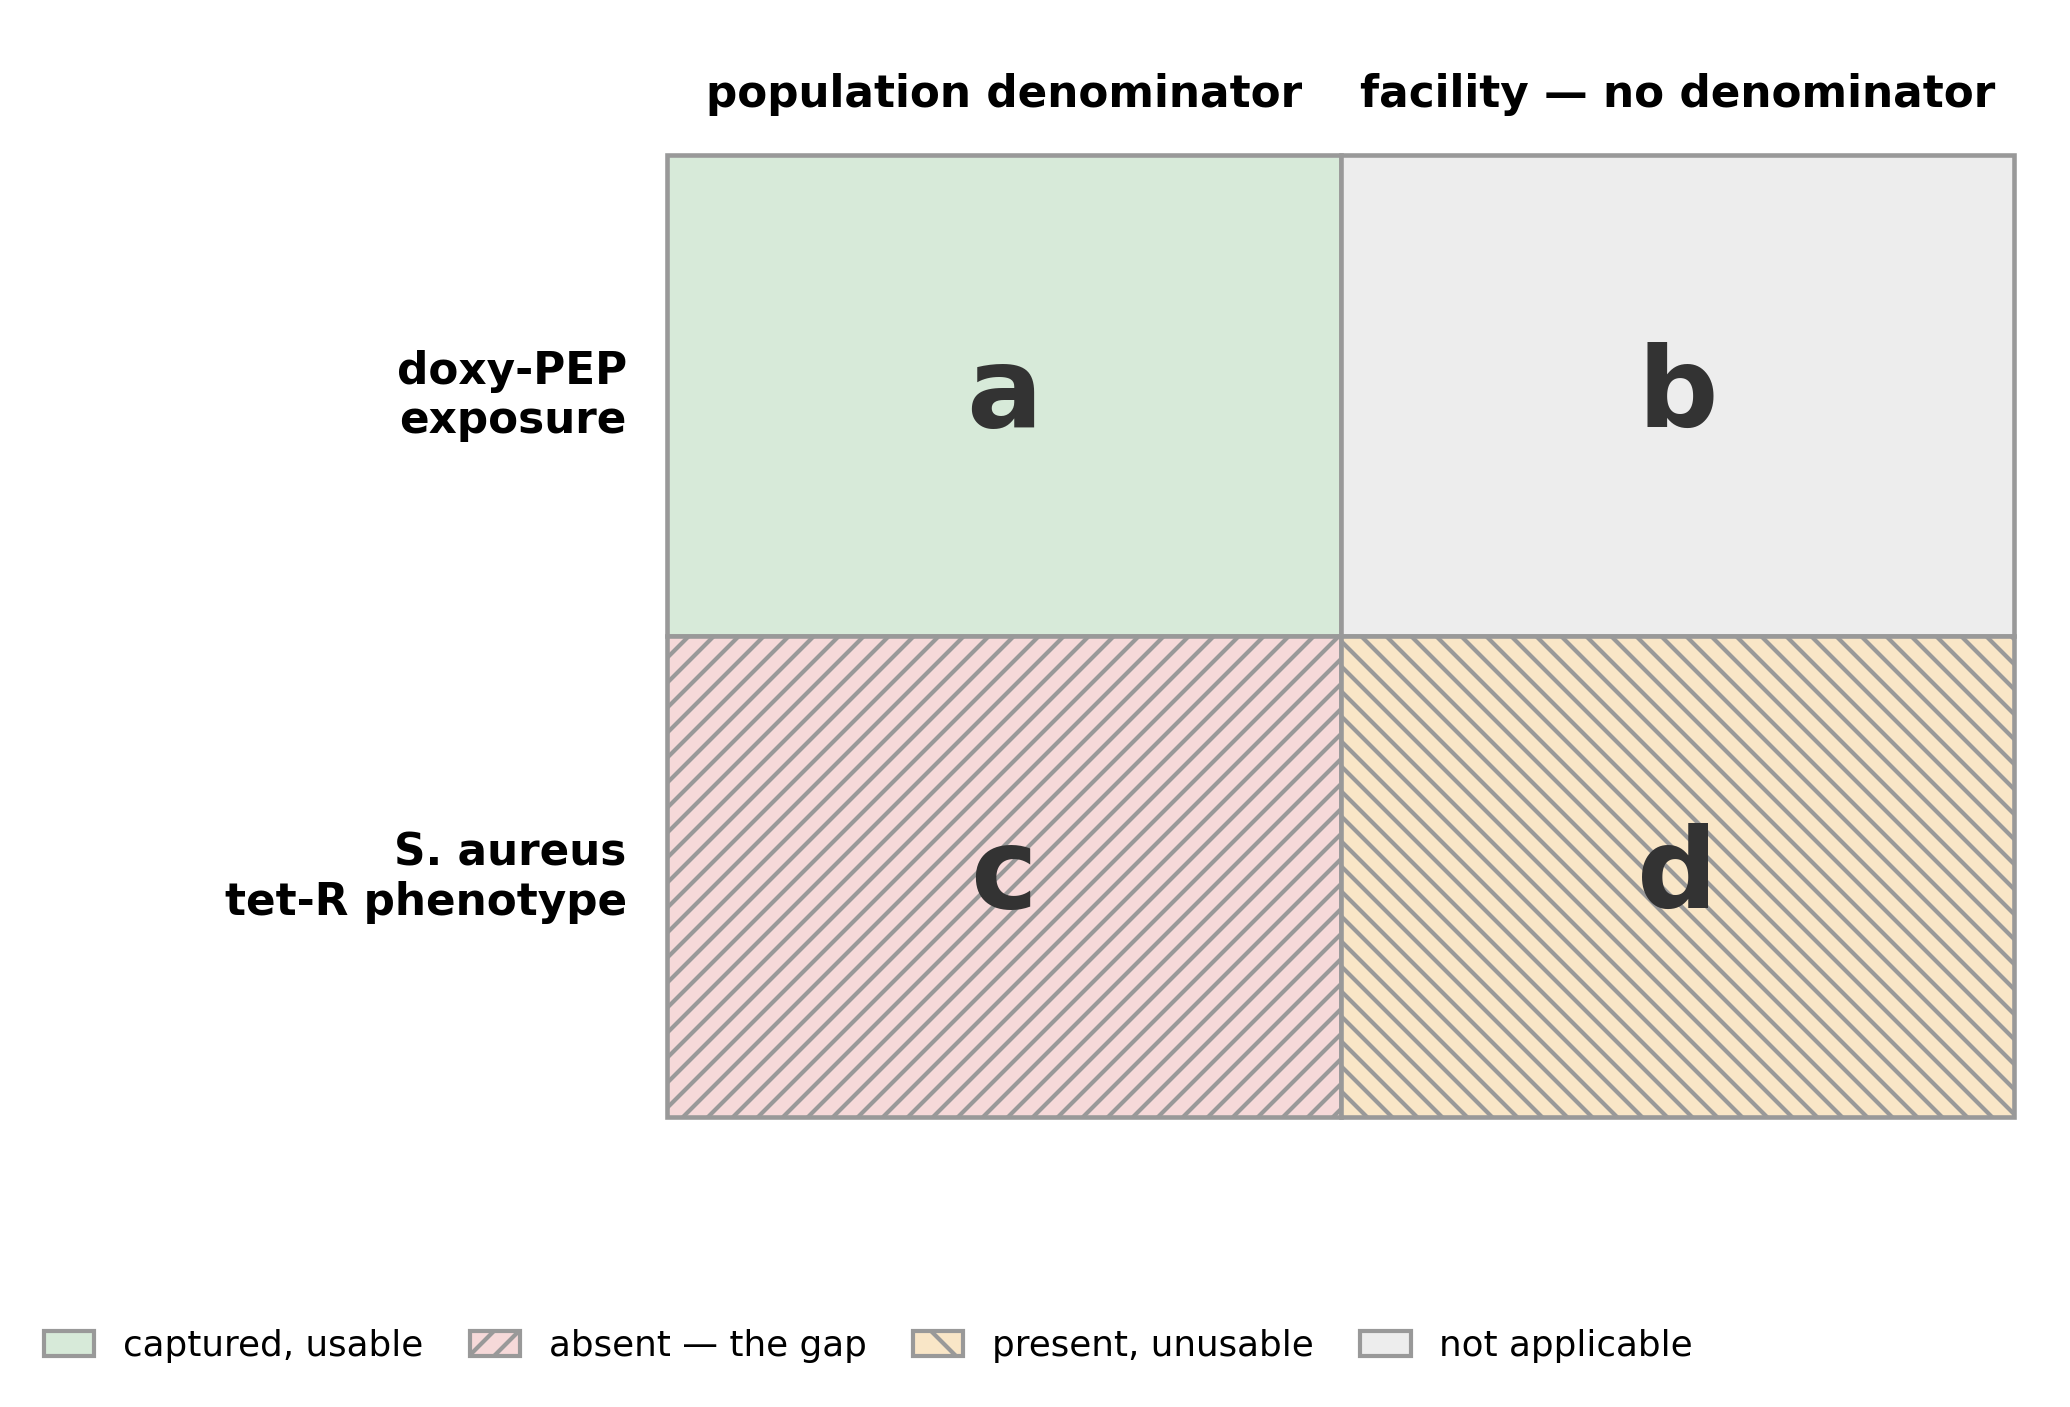
\includegraphics[width=0.9\textwidth]{streamc_linkage.png}
\caption{Surveillance architecture for doxy-PEP exposure and \emph{Staphylococcus aureus} tetracycline resistance.
Schematic summary of the 12 US surveillance and data systems assessed. Each quadrant represents the intersection of the measurement target (rows) and denominator structure (columns): (a) doxy-PEP exposure at a population denominator---captured, although only through PrEP-based proxies (AIDSVu and CDC AtlasPlus); (b) doxy-PEP exposure in facility-level data without a population denominator---not applicable to the population-level linkage question; (c) \emph{S. aureus} tetracycline phenotype at a population denominator---absent, constituting the principal surveillance gap; and (d) \emph{S. aureus} tetracycline phenotype in facility-level data---present in cumulative antibiograms but unusable for population linkage because no population denominator is retained. No assessed system therefore occupies both (a) and (c) within a common linkage structure, and 0 of 12 systems link doxy-PEP exposure to \emph{S. aureus} tetracycline phenotype at a common population denominator.}
\label{fig:linkage}
\end{figure}
\noindent Alt text: A schematic summarising the 12-system surveillance audit:
exposure is captured only as a PrEP proxy and the \sa{} tetracycline phenotype at
a population denominator nowhere, so no system links exposure to phenotype.

\begin{figure}[t]
\centering

\includegraphics[width=0.9\textwidth]{three_streams.png}
\caption{Detectability of the doxy-PEP-associated \emph{S. aureus} resistance signal across the three evidence streams.
The shaded band shows the empirical benchmark range for within-exposed relative risk (RR 1.42--2.25). The final DoxyPEP trial reported a hazard ratio (HR) of 3.89 for incident doxycycline-resistant \emph{S. aureus}. Guidance specifies no \emph{S. aureus} monitoring threshold, whereas modelled population surveillance would require an RR of approximately 6--28 under the primary combined PrEP+PLWH exposure specification; the more restrictive PrEP-only specification requires approximately 14--64. The trial HR is shown only as an empirical magnitude reference and is not numerically interchangeable with the modelled RR thresholds because the estimands differ.}
\label{fig:detect}
\end{figure}
\noindent Alt text: A logarithmic relative-risk axis with a shaded benchmark band
at 1.42 to 2.25; the trial hazard ratio 3.89 sits above the band, surveillance
detectability thresholds of about 6 to 28 (primary combined-denominator
specification; 14 to 64 under the more restrictive PrEP-only specification) sit
far to the right, and guidance has no threshold.

The three streams are summarised against the detectability framework in Table~\ref{tab:audit}; a
PubMed literature-coverage analysis of the bystander organism (361 papers, of
which few name or measure it) is reported in the Supplementary data (S5).

\begin{table}[t]
\centering
\caption{Summary of trial resolution, guidance requirements, and surveillance capability for the doxy-PEP-associated \emph{S. aureus} resistance signal.
The final trial resolved an incident doxycycline-resistant \emph{S. aureus} signal, but no assessed governmental guidance required \emph{S. aureus} monitoring and no assessed US surveillance system linked doxy-PEP exposure to \emph{S. aureus} tetracycline phenotype at a common denominator. RR$_{\text{needed}}$ is the modelled within-exposed relative risk required to produce a detectable population-level change under the primary surveillance specification.}
\label{tab:audit}
\small
\begin{tabularx}{\textwidth}{@{}lXl@{}}
\toprule
Stream & Question & Result\\
\midrule
A. Trials & Was the bystander signal resolved? & Yes---HR 3.89 (1.42--10.68), incident doxy-R \sa{}\\
B. Guidance & Is \sa{} monitoring required? & No---0/6 outbreak-matched; 0/10 coded\\
C. Surveillance & Is exposure linked to phenotype? & No---0/12 systems; RR$_{\text{needed}}\approx$6--28 to detect\\
\bottomrule
\end{tabularx}
\end{table}

% ---------- DISCUSSION ----------
\section*{Discussion}

The pivotal trial has now resolved the bystander question it was long thought
unable to reach: a significant increase in incident doxycycline-resistant \sa{}
under randomised exposure, with no matching effect on carriage, and a call from
its authors for surveillance of exactly this.\cite{luetkemeyer2025} Across the two systems that would have to
receive it---guidance and deployed surveillance---they cannot:
guidance instruments nothing (0/6; 0/10) and no deployed system joins exposure to
the \sa{} tetracycline phenotype at a common denominator (0/12).

The sharper reading is that the trial's measurement system evolved to meet its own
question while the implementation system did not: the same endpoint moved from a
cross-sectional fraction read as reassurance to a participant-level HR of 3.89, yet
guidance and surveillance did not follow\cite{montoya2025estimand}---a demonstrated
signal handed to systems built to measure something else.

\subsection*{Tetracycline resistance mechanisms and the phenotype unit}
Staphylococcal surveillance is standardised around methicillin, yet the
treatment-relevant axis here is tetracycline susceptibility, used empirically
before methicillin status is known, so the two axes are orthogonal. The molecular
basis of tetracycline resistance is likewise heterogeneous: \emph{tet}(K) efflux leaves doxycycline largely
usable whereas \emph{tet}(M) ribosomal protection can compromise it, and the trial
resolved incident doxycycline resistance without resolving
which.\cite{liu2011,grossman2016} Of 823 invasive
USA300 isolates in national surveillance, 72 (9\%) were tetracycline-resistant,
yet 69 were doxycycline-susceptible \emph{tet}(K) and only 3 doxycycline-resistant
\emph{tet}(M)\cite{mcdougal2010}---a single breakpoint that combines mechanisms with opposite implications for
doxycycline susceptibility. An inherited surveillance variable can stay valid for its
original question while being insufficient for the one now imposed on it; we do
not forecast which mechanism is spreading, only that the inherited variable cannot
say.

\subsection*{Instrument requirements for population monitoring}
Following the signal to the population requires an exposure-linked sentinel
instrument the deployed architecture does not provide. Such an instrument would
sample \sa{} from doxy-PEP-exposed individuals, fixing the exposed fraction and the
denominator, and would include the oropharyngeal and peri-anal sites, since
nares-only screening under-detects colonisation by about 20\% in this
population.\cite{kyaw2012} It would report resistance per carrier and by mechanism
(\emph{tet}(M) versus \emph{tet}(K)) rather than as a pooled tetracycline-class
rate, and record dosing frequency rather than prescription status. Finally, it
would carry \sa{} tetracycline susceptibility at a population denominator---most
directly by adding it to the platform that already tracks invasive MRSA---joined to
exposure on geography, with access to individual-level trial data. These components
are technically feasible but are not deployed together at scale.

England's national doxy-PEP monitoring plan is an instructive out-of-frame case. Outside our prespecified US corpus, it nonetheless proposes the phenotype
half we find nowhere---tetracycline resistance in bystander pathogens including
\sa{}---through routine laboratory AMR surveillance.\cite{ukhsa2026} Yet its
specimens come mainly from hospitalised patients; it records neither doxy-PEP use
nor sexual orientation; and its exposure contrast is therefore a male-to-female
resistance ratio in an 18--45 age band, an STI-surveillance conditioning set
carried onto an organism that does not respect it. The same programme already runs
exposure-linked sentinel surveillance that records recent doxy-PEP use---but only
for the gonococcus: the instrument exists, and inheritance points it at the
in-category organism.

These failures share a structure. A guideline or a surveillance system carries in
its sampling frame, cadence, coding, denominator and unit the organism and
question it was built for. The doxy-PEP apparatus, built to measure gonococcal
efficacy, inherits for the bystander commensal a denominator the intervention
itself moves, a phenotype label spanning two mechanisms and a surveillance
architecture standardised around methicillin. We call this \emph{measurement inheritance}. A downstream system
retains the measurement dimensions appropriate to the upstream
question---estimand, denominator, unit, cadence, linkage, measurement
responsibility---but not those the downstream question requires. The question then
becomes unanswerable not for want of data but for want of an inherited dimension.
The construct is built from familiar parts but concerns how they couple
\emph{across} stages of an evidence
chain.\cite{tancredi2024surveillance,treem2023visibility} The downstream gap is
therefore not closable by a better analysis of the trial's data---that analysis has
been done, and it is significant---but is a property of the guidance and
surveillance instruments.

Doxy-PEP's benefit accrues to the recipient; the tetracycline selection cost
falls on people outside the prescribing decision---outpatients with skin
infections and, at the sharp end, dialysis, surgical and oncology patients for whom
the loss of an oral anti-staphylococcal option is consequential. A negative externality that
no deployed instrument can price is not thereby small; it is unweighable. The
wider distributive argument---that the two sides are observed on unequal terms, a
property we term \emph{distributive observability}---is developed in the
Supplementary data (S6).\cite{montoya2025affected}

\subsection*{Limitations}
We make no population-level causal claim and no transmission claim: whether the
individual-level signal propagates into a population externality is precisely what
no deployed system can determine. We did not re-estimate or dispute the trial's randomised result. Colonisation is not
infection, and the colonisation--infection link is itself unmeasured here. Much of
the evidence for how \sa{} clusters and moves through these networks exists only
for its MRSA subset, so where our clustering analysis relies on MRSA we mark it as such. Finally,
the trial reaches only a roughly twelve-month horizon; persistence, dose--response
and mechanism remain open. Our coding carries two asymmetries. The guidance corpus was
double-coded on a 5-document subsample by two passes run through different
interfaces---a command-line agent and a chat interface---but the same model
family, so their errors are not independent; the 92\% concordance measures the
reproducibility of the coding protocol, not its accuracy. The surveillance
enumeration was coded by a single pass. Consistent with a
falsification standard set in advance, the inheritance claim fails if a doxy-PEP
guideline comes to require
\sa{} monitoring, or if a deployed system comes to link doxy-PEP exposure to an
\sa{} tetracycline phenotype at a common population denominator; a proposed
national programme does not yet meet this standard.\cite{ukhsa2026}

\subsection*{Conclusions}
The randomised instrument generated a bystander-resistance signal that the
guidance and surveillance built around doxy-PEP are not instrumented to follow.
The gap is one of measurement architecture, not of missing data, and it is
closable---by sentinel surveillance that links doxy-PEP exposure to the \sa{}
tetracycline phenotype at a common denominator. Until it is built, the population
question the trial's authors posed cannot be answered.

% ---------- BACK MATTER ----------
\section*{Acknowledgements}
A large language model was used for writing and analysis-engineering assistance
beyond copyediting. The scientific argument, the reading of primary sources, the
model specification and all conclusions are the author's own; the author reviewed
all generated content, independently verified every numerical value and quotation
against primary sources and the regenerable analysis outputs, and takes full
responsibility. No artificial-intelligence tool is credited as an author.

\section*{Funding}
This work received no specific grant from any funding agency in the public,
commercial or not-for-profit sectors. It was conducted as an unfunded
investigator-initiated study.

\section*{Transparency declarations}
A.~C.~D. reports former employment at Gilead Sciences (2020--2024) with prior
ownership of corporate stock, all divested by 2024; Gilead played no role in this
work. A.~C.~D. is sole owner of Nyx Dynamics, LLC. No other conflicts to declare.
All data are public (AIDSVu; published trials and guidelines) and all analysis
code is openly available (\url{https://github.com/Nyx-Dynamics/doxypep-bystander})
and archived at Zenodo (doi:\url{10.5281/zenodo.22747669}),\cite{demidont2026compendium}
regenerating every figure
and table by a single command; every coded source is SHA-256-pinned. No
restricted-access data were used.

\bibliography{references}

\end{document}
